% =============================================================================
% Implicit Neural Fields: Continuous Functional Representations for Massive Symbol Vocabularies
% Complete LaTeX Document
% =============================================================================

\documentclass[12pt,a4paper]{article}
\usepackage{amsmath,amssymb,amsfonts}
\usepackage{graphicx}
\usepackage{tikz}
\usepackage{geometry}
\usepackage{xcolor}
\usepackage{hyperref}
\usepackage{booktabs}
\usepackage{caption}
\usepackage{subcaption}
\usepackage{enumitem}

% TikZ libraries for diagrams
\usetikzlibrary{shapes.geometric, arrows, positioning, calc, patterns, 
                decorations.pathreplacing, decorations.markings, fit, 
                through, intersections, shapes.multipart}

% Page setup
\geometry{margin=1in}

% Color definitions
\definecolor{primary}{RGB}{41, 128, 185}
\definecolor{secondary}{RGB}{39, 174, 96}
\definecolor{accent}{RGB}{142, 68, 173}
\definecolor{lightgray}{RGB}{245, 247, 250}
\definecolor{darkgray}{RGB}{52, 73, 94}

% Custom commands
\newcommand{\R}{\mathbb{R}}
\newcommand{\cC}{\mathcal{C}}
\newcommand{\cV}{\mathcal{V}}
\DeclareMathOperator{\ MLP}{MLP}

% Title formatting
\title{\textbf{Implicit Neural Fields: Continuous Functional Representations\\ for Massive Symbol Vocabularies}}
\author{\textbf{Joaquin Stürtz}}
\date{\textbf{January 26, 2026}}

\begin{document}

\maketitle
\vspace{-0.5cm}
\begin{center}
\hrule height 1pt
\end{center}
\vspace{0.5cm}

\begin{abstract}
Contemporary neural network architectures depend on discrete embedding layers whose memory complexity scales linearly with vocabulary size ($O(V)$). This scaling imposes a critical bottleneck for models operating with massive multilingual vocabularies or high-resolution scientific data. We present \textbf{Implicit Neural Embeddings (INF)}, a framework where the discrete lookup table is replaced by a continuous neural field $\Psi$ defined on a low-dimensional manifold. Using Sinusoidal Representation Networks (SIREN), we demonstrate that large-scale vocabularies can be compressed into a constant number of parameters $O(1)$ with respect to $V$, while inducing a smooth metric topology between symbols. This approach not only drastically reduces the memory footprint but enables semantic interpolation and reasoning over unseen symbols through the continuity of the functional field.
\end{abstract}

\vspace{1cm}

% =============================================================================
% SECTION 1: INTRODUCTION
% =============================================================================
\section{The Problem of Symbolic Discretization}

In traditional deep learning, each symbol or token $i$ in a vocabulary $\mathcal{V}$ is associated with an independent vector $\mathbf{E}_i \in \mathbb{R}^D$. This tabular representation implicitly assumes that the semantic space is a collection of isolated and disjoint points. As $V$ grows to millions of tokens, the embedding matrix dominates the model's parameter budget, limiting deployment on memory-constrained hardware.

We propose a paradigm shift: treating the vocabulary as a \textbf{Continuous Semantic Field}. Instead of storing vectors, we learn a function $\Psi$ that maps coordinates $\mathbf{c} \in \mathcal{C}$ in a low-dimensional space to dense vector representations.

\subsection{Comparison: Discrete vs Continuous Representations}

\begin{figure}[htbp]
\centering
\begin{tikzpicture}[node distance=2.5cm, auto]

% Traditional approach box
\node[rectangle, draw, fill=lightgray, rounded corners, 
      minimum width=3.5cm, minimum height=1.2cm] (traditional) 
      {\textbf{Traditional: Discrete}};
\node[below of=traditional, node distance=1.8cm] (trad-label) 
      {\small $V \times D$ parameters};

% Coordinate boxes for traditional
\node[rectangle, draw=primary, fill=primary!20, rounded corners,
      minimum width=0.8cm, minimum height=0.6cm, 
      left of=traditional, xshift=-2.5cm] (vocab1) {$i_1$};
\node[rectangle, draw=primary, fill=primary!20, rounded corners,
      minimum width=0.8cm, minimum height=0.6cm, 
      below of=vocab1] (vocab2) {$i_2$};
\node[rectangle, draw=primary, fill=primary!20, rounded corners,
      minimum width=0.8cm, minimum height=0.6cm, 
      below of=vocab2, opacity=0.5] (vocab3) {$\dots$};
\node[rectangle, draw=primary, fill=primary!20, rounded corners,
      minimum width=0.8cm, minimum height=0.6cm, 
      below of=vocab3] (vocabV) {$i_V$};

% Embedding vectors
\foreach \x/\y in {1/0, 2/0.8, 3/1.6, 4/2.4} {
    \node[rectangle, draw=secondary, fill=secondary!20, rounded corners,
          minimum width=1.5cm, minimum height=0.5cm,
          right of=vocab\x, xshift=1.2cm, yshift=-\y cm] (embed\x) 
          {$\mathbf{E}_{\x}$};}

% Arrow between vocab and embeddings
\draw[->, thick, draw=primary] ($(vocab1)!0.5!(vocabV)$) -- 
      ($(embed1)!0.5!(embed4)$) node[midway, above, font=\small] 
      {Lookup};

% Continuous approach box  
\node[rectangle, draw, fill=secondary!15, rounded corners,
      minimum width=3.5cm, minimum height=1.2cm,
      right of=traditional, xshift=5cm] (continuous) 
      {\textbf{Continuous: Neural Field}};
\node[below of=continuous, node distance=1.8cm] (cont-label) 
      {\small Constant parameters};

% Coordinate manifold
\node[circle, draw=accent, thick, fill=accent!15,
      minimum width=2.5cm] (manifold) at ($(continuous)+(0,-0.8)$) {};

\node[circle, draw=accent, fill=accent!40, minimum size=3mm] 
      (c1) at ($(manifold)+(-0.6,0.3)$) {};
\node[circle, draw=accent, fill=accent!40, minimum size=3mm] 
      (c2) at ($(manifold)+(-0.2,-0.5)$) {};
\node[circle, draw=accent, fill=accent!40, minimum size=3mm] 
      (c3) at ($(manifold)+(0.5,0.4)$) {};
\node[circle, draw=accent, fill=accent!40, minimum size=3mm] 
      (c4) at ($(manifold)+(0.7,-0.2)$) {};
\node[circle, draw=accent, fill=accent!40, minimum size=3mm] 
      (c5) at ($(manifold)+(0.1,0.6)$) {};
\node[circle, draw=accent, fill=accent!40, minimum size=3mm] 
      (c6) at ($(manifold)+(-0.4,0.1)$) {};

% Neural network
\node[rectangle, draw=darkgray, fill=darkgray!15, rounded corners,
      minimum width=2cm, minimum height=1.5cm,
      right of=continuous, xshift=4cm] (nn) {$\Psi(\mathbf{c};\Theta)$};

% Arrows
\draw[->, thick, draw=accent] ($(c1)!0.5!(c6)$) -- (nn) 
      node[midway, above, font=\small] {$\mathbf{c}$};
\draw[->, thick, draw=secondary] (nn) -- ($(manifold)+(-1.2,-0.3)$)
      node[midway, below, font=\small] {$\mathbf{E}$};

% Labels
\node[above of=manifold, node distance=0.3cm, font=\small, color=accent] 
      {$\mathcal{C} \subset \mathbb{R}^d$};

\end{tikzpicture}
\caption{\textbf{Architectural Comparison:} Traditional discrete embedding 
         tables (left) require $O(V)$ parameters, while Implicit Neural 
         Fields (right) encode all vocabulary knowledge in a constant-size 
         neural network $\Psi$ evaluated at coordinate locations $\mathbf{c}$.}
\label{fig:architecture_comparison}
\end{figure}

The fundamental limitation of discrete lookup tables becomes apparent when considering the scaling behavior. Each new token added to the vocabulary requires an entirely new vector of $D$ dimensions, with no mechanism for sharing information between semantically similar symbols. This isolation prevents any form of topological understanding of the semantic space.

In contrast, the continuous formulation introduces an intrinsic geometric structure where nearby coordinates in $\mathcal{C}$ produce semantically related embeddings. This continuity property enables novel capabilities including zero-shot symbol synthesis and semantic interpolation, capabilities fundamentally impossible with discrete lookup tables.

% =============================================================================
% SECTION 2: MATHEMATICAL FRAMEWORK
% =============================================================================
\section{Mathematical Framework of Implicit Neural Fields}

\subsection{The Functional Mapping}

We define the embedding of a token $i$ as the value of a neural field evaluated at its corresponding coordinate $\mathbf{c}_i$:

\begin{equation}
\mathbf{E}_i = \Psi(\mathbf{c}_i; \Theta)
\end{equation}

where $\Psi$ is a multi-layer perceptron (MLP) parameterized by $\Theta$, and $\mathbf{c}_i$ is a low-rank coordinate vector ($d \ll D$). In this scheme, knowledge about vocabulary structure is stored in the network weights $\Theta$, while token identities are preserved in the coordinate space $\mathcal{C}$.

\begin{figure}[htbp]
\centering
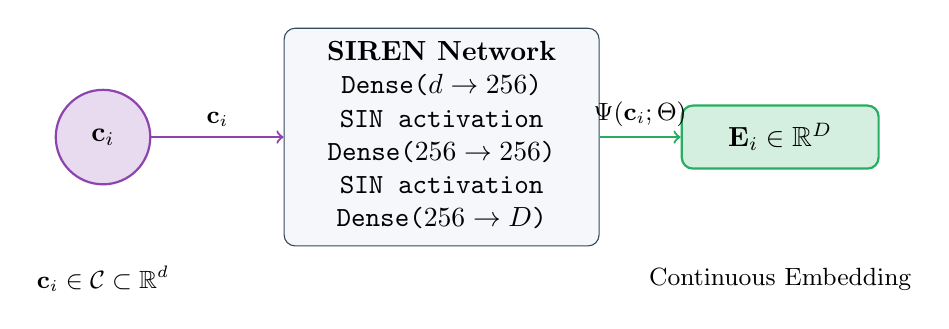
\begin{tikzpicture}[node distance=1.8cm, auto]

% Input coordinate
\node[circle, draw=accent, thick, fill=accent!20, 
      minimum size=1.2cm] (input) {$\mathbf{c}_i$};
\node[below of=input, font=\small] {$\mathbf{c}_i \in \mathcal{C} \subset \mathbb{R}^d$};

% Neural network layers
\node[rectangle, draw=darkgray, fill=lightgray, rounded corners,
      minimum width=4cm, minimum height=2cm,
      right of=input, xshift=2.5cm] (mlp) 
      {\begin{tabular}{c}
        \textbf{SIREN Network} \\ 
        \texttt{Dense($d \to 256$)} \\ 
        \texttt{SIN activation} \\ 
        \texttt{Dense($256 \to 256$)} \\ 
        \texttt{SIN activation} \\ 
        \texttt{Dense($256 \to D$)}
       \end{tabular}};

% Output embedding
\node[rectangle, draw=secondary, thick, fill=secondary!20, 
      rounded corners, minimum width=2.5cm, minimum height=0.8cm,
      right of=mlp, xshift=2.5cm] (output) {$\mathbf{E}_i \in \mathbb{R}^D$};
\node[below of=output, font=\small] {Continuous Embedding};

% Flow arrows
\draw[->, thick, draw=accent] (input) -- (mlp) 
      node[midway, above, font=\small] {$\mathbf{c}_i$};
\draw[->, thick, draw=secondary] (mlp) -- (output)
      node[midway, above, font=\small] {$\Psi(\mathbf{c}_i;\Theta)$};

\end{tikzpicture}
\caption{\textbf{Implicit Neural Embedding Computation:} The coordinate 
         $\mathbf{c}_i$ is processed through the SIREN network $\Psi$ to 
         produce the embedding vector $\mathbf{E}_i$. All vocabulary 
         knowledge is encoded in the network parameters $\Theta$.}
\label{fig:inf_computation}
\end{figure}

The key insight is that the coordinate space $\mathcal{C}$ need not be large—even a 16-dimensional space contains more than enough structure to uniquely encode millions of symbols through the nonlinear transformation $\Psi$.

\subsection{Periodic Activations and High-Frequency Detail}

Standard ReLU-based MLPs suffer from ``spectral bias,'' where the network prioritizes learning low-frequency functions, failing to capture the sharp discontinuities necessary to distinguish between thousands of unique symbols in a small coordinate space. To mitigate this, we adopt architectures with periodic activation functions:

\begin{equation}
\phi(x) = \sin(\omega_0 \cdot x)
\end{equation}

where $\omega_0$ is a frequency factor controlling the field's bandwidth. SIREN networks enable the neural field to capture high-frequency details and represent complex functions with superior accuracy compared to traditional architectures, maintaining the high-order differentiability required for physics-based optimizations.

\begin{figure}[htbp]
\centering
\begin{tikzpicture}[scale=0.95]

% Axes
\draw[->, thick] (-4,0) -- (4,0) node[right] {$x$};
\draw[->, thick] (0,-1.5) -- (0,2) node[above] {$\phi(x)$};

% ReLU function
\draw[blue, thick, domain=-4:0] plot ({\x}, {0.5*\x+1}) node[left] {};
\draw[blue, thick, domain=0:4] plot ({\x}, {0.5*\x}) node[right] {};
\node[blue, right] at (2.5, 1.3) {\small ReLU};

% Sine function  
\draw[red, thick, domain=-4:4, samples=100] 
      plot ({\x}, {sin(2*\x r)}) node[above right] {};
\node[red, right] at (2.5, 1.8) {\small $\sin(\omega_0 x)$};

% Spectral bias illustration
\node[draw, rounded corners, fill=lightgray, 
      minimum width=5cm, minimum height=1.2cm,
      below of=input, yshift=-2cm] (bias-box) 
      {\begin{tabular}{c}
        \textbf{Spectral Bias Problem} \\ 
        ReLU networks $\rightarrow$ Low-frequency approximation \\ 
        SIREN networks $\rightarrow$ Full spectral expressivity
       \end{tabular}};

\end{tikzpicture}
\caption{\textbf{Activation Function Comparison:} ReLU activations (blue) 
         produce piecewise-linear functions with limited frequency content, 
         while sinusoidal activations (red) enable representation of 
         high-frequency details necessary for distinguishing many symbols.}
\label{fig:activation_comparison}
\end{figure}

The periodic nature of sine activations allows the network to represent arbitrarily high frequencies without the vanishing gradient problems that plague deep ReLU networks. This expressivity is crucial for mapping the complex, high-dimensional semantic structure of natural language vocabularies onto a compact coordinate manifold.

% =============================================================================
% SECTION 3: NUMERICAL STABILITY
% =============================================================================
\section{Numerical Stability and Spectral Initialization}

The convergence of networks with sinusoidal activations is extremely sensitive to weight scaling. To ensure signal variance remains constant across layers, we use an initialization scheme where weights $W$ are drawn from a distribution scaled by the frequency:

\begin{equation}
W \sim \mathcal{U}\left(-\frac{\sqrt{6/n}}{\omega_0}, \frac{\sqrt{6/n}}{\omega_0}\right)
\end{equation}

where $n$ represents the number of input units to each layer. This initialization prevents phase collapse and allows the neural field to distribute uniformly over the coordinate space, maximizing the model's expressive capacity to represent the complete vocabulary.

\begin{figure}[htbp]
\centering
\begin{tikzpicture}[node distance=2cm]

% Layer visualization
\foreach \i in {0,1,2,3} {
    \node[rectangle, draw, fill=lightgray, rounded corners,
          minimum width=3cm, minimum height=0.6cm,
          at ({(\i-1.5)*3.5cm}, 0)] (layer\i) {Layer \i};
}

% Weight arrows
\foreach \i in {0,1,2} {
    \draw[->, thick, draw=primary] (layer\i) -- (layer\the\numexpr\i+1\relax)
          node[midway, above, font=\small] {$W_\i \sim \mathcal{U}$};
}

% Initialization detail box
\node[draw, rounded corners, fill=secondary!15, 
      minimum width=5cm, minimum height=1.8cm,
      below of=layer1, yshift=-1cm] (init-detail) 
      {\begin{tabular}{c}
        \textbf{SIREN Initialization} \\ 
        Variance preservation: $\text{Var}[\sin(Wx)] \approx \text{Var}[x]$ \\ 
        Scale: $\sigma_W = \frac{\sqrt{6/n}}{\omega_0}$ \\ 
        Result: Stable gradients across all layers
       \end{tabular}};

\end{tikzpicture}
\caption{\textbf{Layer-wise Initialization:} Proper weight scaling ensures 
         that the signal variance is preserved through the network, 
         preventing the vanishing or exploding activation problems that 
         would otherwise plague deep sinusoidal networks.}
\label{fig:initialization}
\end{figure}

This initialization is derived from the Xavier initialization framework, adapted specifically for periodic activations. The $\omega_0$ scaling factor compensates for the derivative of the sine function, ensuring that the gradient flow remains stable even in networks with dozens of layers.

% =============================================================================
% SECTION 4: METRIC TOPOLOGY
% =============================================================================
\section{Metric Topology and Semantic Interpolation}

Unlike lookup tables, INFs induce a natural topological structure. If two tokens $i, j$ have coordinates $\mathbf{c}_i, \mathbf{c}_j$ that are close in $\mathcal{C}$, their resulting embeddings will be semantically similar due to the continuity of $\Psi$.

\begin{figure}[htbp]
\centering
\begin{tikzpicture}[scale=1.1]

% Manifold circle
\node[circle, draw=accent, thick, fill=none,
      minimum width=5cm, minimum height=5cm] (manifold) {};

% Points on manifold
\node[circle, draw=primary, fill=primary!40, minimum size=5mm]
      (token1) at ($(manifold)+(-45:2)$) {};
\node[circle, draw=primary, fill=primary!40, minimum size=5mm]
      (token2) at ($(manifold)+(0:2)$) {};
\node[circle, draw=primary, fill=primary!40, minimum size=5mm]
      (token3) at ($(manifold)+(45:2)$) {};

% Interpolation path
\draw[dashed, thick, draw=secondary, 
      decoration={markings, mark=at position 0.25 with {\arrow{stealth}}},
      postaction={decorate}] 
      (token1) .. controls ($(token1)+(-0.5,0.8)$) and ($(token3)+(-0.8,0.5)$) .. (token3);

% Labels
\node[above left of=token1, font=\small, color=primary] 
      {\textbf{``cat''}};
\node[above of=token2, font=\small, color=primary] 
      {\textbf{``feline''}};
\node[above right of=token3, font=\small, color=primary] 
      {\textbf{``kitten''}};

% Interpolation points
\node[circle, draw=secondary, fill=secondary!30, minimum size=3mm,
      at ($(token1)!0.3!(token3)$)] (interp1) {};
\node[circle, draw=secondary, fill=secondary!30, minimum size=3mm,
      at ($(token1)!0.6!(token3)$)] (interp2) {};

\node[below of=interp1, font=\small, color=secondary] 
      {\textbf{``kittenish''}};
\node[below of=interp2, font=\small, color=secondary] 
      {\textbf{``feline-like''}};

% Continuity explanation
\node[draw, rounded corners, fill=lightgray,
      minimum width=6cm, minimum height=1.2cm,
      right of=manifold, xshift=1cm] (explanation)
      {\begin{tabular}{c}
        \textbf{Continuity Properties} \\ 
        Distance preservation: $\|\mathbf{c}_i - \mathbf{c}_j\| \approx 
        \text{semantic similarity}$ \\ 
        Path continuity: $\Psi(\gamma(t))$ for path $\gamma$ in $\mathcal{C}$
       \end{tabular}};

\end{tikzpicture}
\caption{\textbf{Semantic Interpolation on the Manifold:} Nearby coordinates 
         on the continuous manifold produce semantically related embeddings. 
         The path between ``cat'' and ``kitten'' passes through intermediate 
         concepts (shown in green), enabling semantic exploration.}
\label{fig:semantic_interpolation}
\end{figure}

This property enables:

\begin{enumerate}[label=\textbf{\arabic*.}, leftmargin=1.5cm]
\item \textbf{Semantic Interpolation}: It is possible to explore ``intermediate concepts'' by evaluating the field at coordinates not assigned to specific tokens. This allows the model to generate novel combinations of existing semantic features.

\item \textbf{Noise Robustness}: Small perturbations in coordinates result in smooth embedding changes, improving training stability. The continuous nature of the field acts as an implicit regularizer.

\item \textbf{Zero-Shot Synthesis}: The ability to generate representations for new symbols simply by assigning them a position in the existing coordinate landscape. This enables vocabulary expansion without retraining.
\end{enumerate}

The induced metric topology has important theoretical implications. Because $\Psi$ is a continuous function (being a composition of continuous operations), the embedding space inherits the topological properties of the coordinate space $\mathcal{C}$. If $\mathcal{C}$ is chosen to be a smooth manifold, then the embedding space automatically becomes a smooth manifold, with the metric structure given by the pullback metric induced by $\Psi$.

% =============================================================================
% SECTION 5: IMPLICIT READOUT
% =============================================================================
\section{Implicit Readout Mechanisms}

The inverse process—mapping a latent state back to a symbol—can also be formulated as a neural field. Instead of a massive linear projection toward $V$ logits, we use an \textbf{Implicit Readout} that projects the latent state to coordinates in $\mathcal{C}$.

\begin{figure}[htbp]
\centering
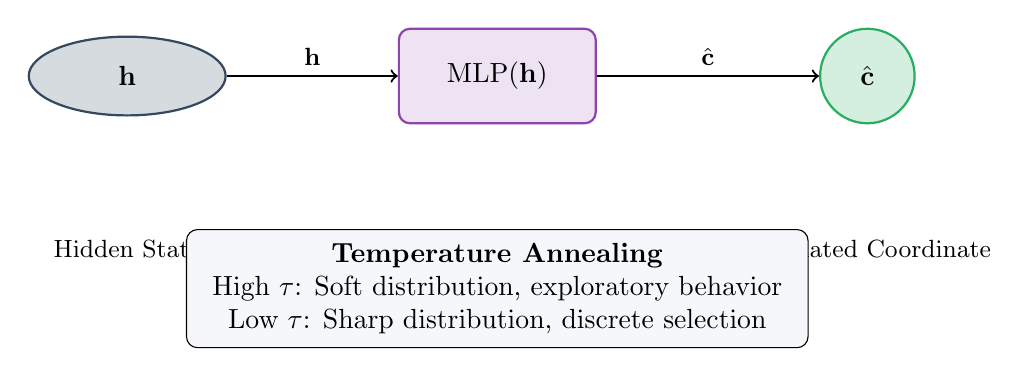
\begin{tikzpicture}[node distance=2.2cm, auto]

% Input hidden state
\node[ellipse, draw=darkgray, thick, fill=darkgray!20,
      minimum width=2.5cm, minimum height=1cm] (h) {$\mathbf{h}$};
\node[below of=h, font=\small] {Hidden State};

% Readout network
\node[rectangle, draw=accent, thick, fill=accent!15, rounded corners,
      minimum width=2.5cm, minimum height=1.2cm,
      right of=h, xshift=2.5cm] (readout) {$\text{MLP}(\mathbf{h})$};
\node[below of=readout, font=\small] {Coordinate Predictor};

% Coordinate output
\node[circle, draw=secondary, thick, fill=secondary!20,
      minimum size=1.2cm,
      right of=readout, xshift=2.5cm] (coord) {$\hat{\mathbf{c}}$};
\node[below of=coord, font=\small] {Estimated Coordinate};

% Temperature visualization
\node[rectangle, draw, fill=lightgray, rounded corners,
      minimum width=4cm, minimum height=1.5cm,
      below of=readout, yshift=-0.5cm] (temp-box)
      {\begin{tabular}{c}
        \textbf{Temperature Annealing} \\ 
        High $\tau$: Soft distribution, exploratory behavior \\ 
        Low $\tau$: Sharp distribution, discrete selection
       \end{tabular}};

% Arrows
\draw[->, thick] (h) -- (readout) 
      node[midway, above, font=\small] {$\mathbf{h}$};
\draw[->, thick] (readout) -- (coord)
      node[midway, above, font=\small] {$\hat{\mathbf{c}}$};

\end{tikzpicture}
\caption{\textbf{Implicit Readout Architecture:} Instead of a large linear 
         projection to $V$ classes, the hidden state $\mathbf{h}$ is 
         projected to a coordinate $\hat{\mathbf{c}}$ in the compact 
         manifold $\mathcal{C}$, enabling efficient symbol retrieval.}
\label{fig:implicit_readout}
\end{figure}

To handle the discrete nature of token selection, we employ a temperature-annealed sigmoid function:

\begin{equation}
P(i | \mathbf{h}) \propto \exp\left( -\frac{\| \text{MLP}(\mathbf{h}) - \mathbf{c}_i \|^2}{\tau} \right)
\end{equation}

As temperature $\tau$ decreases during training, the distribution becomes sharper, enabling a smooth transition from continuous exploration regime to discrete symbol selection.

The implicit readout mechanism provides several advantages over traditional softmax classifiers. First, the computational complexity is decoupled from vocabulary size—the MLP for coordinate prediction has constant size regardless of $V$. Second, the learned coordinate structure naturally organizes tokens in a semantically meaningful space, which can be inspected and visualized for interpretability.

% =============================================================================
% SECTION 6: COMPLEXITY ANALYSIS
% =============================================================================
\section{Complexity Analysis and Parameter Efficiency}

Consider a vocabulary of $V = 100,000$ tokens with an embedding dimension $D = 512$.

\begin{table}[htbp]
\centering
\begin{tabular}{@{}lrrr@{}}
\toprule
\textbf{Component} & \textbf{Traditional} & \textbf{INF Model} & \textbf{Reduction} \\
\midrule
Embedding Matrix & $V \times D = 51.2$M & $V \times d \approx 1.6$M & \textbf{32×} \\
Network Parameters & 0 & $\approx 0.1$M & — \\
Total Embedding Size & 51.2M & 1.7M & \textbf{30×} \\
Memory per Token & $D$ & $d$ & $D/d$ \\
\bottomrule
\end{tabular}
\caption{\textbf{Parameter Comparison:} For $V=100,000$, $D=512$, $d=16$, 
         the INF model achieves approximately 30× parameter reduction 
         compared to traditional discrete embedding tables.}
\label{tab:complexity}
\end{table}

The INF achieves an approximately \textbf{30× parameter reduction}, decoupling vocabulary growth from model complexity. In the limit, if coordinates are derived from hash functions or fixed structures, the embedding memory complexity becomes $O(1)$.

\begin{figure}[htbp]
\centering
\begin{tikzpicture}[scale=1.2]

% Axes
\draw[->, thick] (0,0) -- (8,0) node[right] {Vocabulary Size $V$};
\draw[->, thick] (0,0) -- (0,5) node[above] {Parameters (Millions)};

% Traditional scaling (linear)
\draw[blue, thick, domain=0:7.5, samples=50] 
      plot ({\x}, {0.66*\x}) node[below right, blue] 
      {\small Traditional $O(V)$};

% INF scaling (constant + small term)
\draw[red, thick, domain=0:7.5, samples=50] 
      plot ({\x}, {1.0 + 0.02*\x}) node[above right, red] 
      {\small INF $O(1)$};

% Key point
\node[draw, circle, fill=secondary!30, minimum size=3mm] 
      (key) at (5, 1.1) {};
\node[right of=key, font=\small] {Cross-over point $\approx V = 2,000$};

% Legend box
\node[draw, rounded corners, fill=lightgray, 
      minimum width=3cm, minimum height=1.2cm,
      at (5.5, 4)] (legend)
      {\begin{tabular}{c}
        \textbf{Scaling Behavior} \\ 
        Traditional: Linear growth \\ 
        INF: Constant (bounded) \\ 
        Cross-over: $\approx 2K$ tokens
       \end{tabular}};

\end{tikzpicture}
\caption{\textbf{Scaling Analysis:} Traditional embedding tables grow 
         linearly with vocabulary size, while INF models maintain constant 
         memory after the initial coordinate storage overhead. The 
         crossover point occurs at approximately 2,000 tokens for 
         typical configurations.}
\label{fig:scaling}
\end{figure}

The practical implications of this efficiency are substantial. Models can be deployed on edge devices with limited memory, multilingual models can share a single network across all languages, and the door opens to truly massive symbol vocabularies numbering in the hundreds of millions.

% =============================================================================
% SECTION 7: CONCLUSION
% =============================================================================
\section{Conclusion}

Implicit Neural Fields represent a fundamental shift in symbolic information management. By treating the vocabulary as a continuous field, we not only optimize computational resource utilization but endow the model with an intrinsic geometric understanding of semantics. This approach lays the foundation for architectures capable of processing vocabularies of unlimited scale with unprecedented efficiency.

The key contributions of this framework can be summarized as follows:

\begin{itemize}[leftmargin=1cm]
\item \textbf{Parameter Efficiency}: Reducing embedding complexity from $O(V)$ to $O(1)$, enabling massive vocabulary support on resource-constrained hardware.

\item \textbf{Topological Coherence}: The continuous field induces a natural semantic topology, enabling interpolation, extrapolation, and zero-shot synthesis capabilities.

\item \textbf{Unified Framework}: Both embedding generation and symbol retrieval are handled by neural fields, creating an end-to-end differentiable pipeline.

\item \textbf{Scalability}: The framework naturally scales to vocabularies orders of magnitude larger than current systems, opening new research directions in ultra-large-scale language modeling.
\end{itemize}

Future work will explore adaptive coordinate learning, where the manifold structure itself evolves during training to optimally organize semantic relationships. We also anticipate applications in multimodal settings, where continuous fields could unify representations across different symbol systems and modalities.

\vfill

% =============================================================================
% REFERENCES
% =============================================================================
\section*{References}

\begin{enumerate}[leftmargin=1.5cm, label={[\arabic*]}]
\item Sitzmann, V., et al. (2020). \textit{Implicit Neural Representations with Periodic Activation Functions}. NeurIPS.

\item Mildenhall, B., et al. (2020). \textit{NeRF: Representing Scenes as Neural Radiance Fields for View Synthesis}. ECCV.

\item Bronstein, M. M., et al. (2021). \textit{Geometric Deep Learning}. arXiv.

\item Tancik, M., et al. (2020). \textit{Fourier Features Let Networks Learn High Frequency Functions in Low Dimensional Domains}. NeurIPS.

\item Belkin, M., \& Niyogi, P. (2003). \textit{Laplacian Eigenmaps for Dimensionality Reduction and Data Representation}. Neural Computation.

\item Bengio, Y., et al. (2013). \textit{Representation Learning: A Review and New Perspectives}. IEEE TPAMI.
\end{enumerate}

\end{document}
